\documentclass[11pt,a4paper]{article}

% =============================================
% Packages
% =============================================
\usepackage[utf8]{inputenc}
\usepackage[T1]{fontenc}
\usepackage{amsmath,amssymb,amsthm}
\usepackage{graphicx}
\usepackage{booktabs}
\usepackage{enumitem}
\usepackage{geometry}
\usepackage{setspace}
\usepackage{hyperref}
\usepackage[numbers]{natbib}
\usepackage{xcolor}
\usepackage{fancyhdr}
\usepackage{titlesec}
\usepackage{float}
\usepackage{caption}
\usepackage{tcolorbox}
\usepackage{tabularx}
\usepackage{array}
\usepackage{url}
\urlstyle{tt}

% Public repository (GitHub; Zenodo DOI filled at archival release)
\newcommand{\ExcessThreeRepo}{https://github.com/johelpadilla/excess3}
\newcommand{\ExcessThreeRepoShort}{github.com/johelpadilla/excess3}
\newcommand{\ExcessThreeDOI}{10.5281/zenodo.21385937}
\newcommand{\ExcessThreeDOIURL}{https://doi.org/10.5281/zenodo.21385937}

\geometry{margin=1in}
\onehalfspacing

\titleformat{\section}{\large\bfseries}{\thesection}{0.6em}{}
\titleformat{\subsection}{\normalsize\bfseries}{\thesubsection}{0.5em}{}
\titleformat{\subsubsection}{\normalsize\itshape}{\thesubsubsection}{0.5em}{}

\pagestyle{fancy}
\fancyhf{}
\fancyhead[L]{\small Understanding excess$^3$ --- a cross-disciplinary guide}
\fancyhead[R]{\small \thepage}
\renewcommand{\headrulewidth}{0.4pt}

\hypersetup{
  colorlinks=true,
  linkcolor=blue!60!black,
  citecolor=blue!60!black,
  urlcolor=blue!70!black,
  pdftitle={Understanding excess3: A Cross-Disciplinary Guide to Order-3 Synergistic Surplus},
  pdfauthor={Johel Padilla-Villanueva},
  pdfkeywords={excess3, pedagogy, synergistic information, multivariate dependence, RECD, complex systems}
}

% Callout boxes
\newtcolorbox{keyidea}[1][]{
  colback=blue!4!white,
  colframe=blue!70!black,
  title={\textbf{Key idea}},
  fonttitle=\bfseries,
  boxrule=0.7pt,
  left=4pt,right=4pt,top=2pt,bottom=2pt,
  #1
}
\newtcolorbox{warningbox}[1][]{
  colback=orange!5!white,
  colframe=orange!70!black,
  title={\textbf{Caution}},
  fonttitle=\bfseries,
  boxrule=0.7pt,
  left=4pt,right=4pt,top=2pt,bottom=2pt,
  #1
}
\newtcolorbox{workbox}[1][]{
  colback=green!4!white,
  colframe=green!50!black,
  title={\textbf{Worked example}},
  fonttitle=\bfseries,
  boxrule=0.7pt,
  left=4pt,right=4pt,top=2pt,bottom=2pt,
  #1
}
\newtcolorbox{fieldbox}[1][]{
  colback=purple!4!white,
  colframe=purple!55!black,
  title={\textbf{In your field}},
  fonttitle=\bfseries,
  boxrule=0.7pt,
  left=4pt,right=4pt,top=2pt,bottom=2pt,
  #1
}
\newtcolorbox{defbox}[1][]{
  colback=gray!6!white,
  colframe=gray!55!black,
  title={\textbf{Definition (plain language)}},
  fonttitle=\bfseries,
  boxrule=0.7pt,
  left=4pt,right=4pt,top=2pt,bottom=2pt,
  #1
}

\title{\textbf{Understanding excess$^3$:}\\[0.35em]
A Cross-Disciplinary Guide to Order-3\\
Synergistic Surplus\\[0.55em]
\large How to read, apply, and not over-claim a high-order\\
dependence measure---without requiring a graduate course\\
in information theory}

\author{
Johel Padilla-Villanueva \\
\textit{Department of Environmental Health, University of Puerto Rico} \\
ORCID: \href{https://orcid.org/0000-0002-5797-6931}{0000-0002-5797-6931} \\
\texttt{johelpadilla@gmail.com} \\
\texttt{joel.padilla2@upr.edu}
}

\date{Guide v1.0 \quad | \quad July 2026 \\[0.25em]\small Repository: \href{\ExcessThreeRepo}{\ExcessThreeRepoShort}\\[0.15em]\small DOI: \href{\ExcessThreeDOIURL}{\ExcessThreeDOI}}

\begin{document}
\maketitle

% =============================================
\begin{abstract}
\noindent
Many scientific fields---ecology, epidemiology, physiology, climate science,
neuroscience, and the social sciences---need tools that detect when several
variables reorganise \emph{together} in a way that pairwise correlations
cannot fully explain. That idea is often called \emph{high-order} or
\emph{synergistic} dependence. It is scientifically important and easy to
misread.

This guide introduces \textbf{excess$^3$} (code name \texttt{excess3}): a
pre-specified continuous proxy for order-3 synergistic surplus used in the
Systemic Tau / RECD research programme. It is written for working scientists
who are comfortable with statistics at the level of mutual information or
regression, but who may not specialise in partial information decomposition
(PID) or symbolic dynamics.

We prioritise intuition, analogies, and step-by-step calculation over
brevity. Formal proofs, full synthetic batteries, and software edge cases are
left to the methods paper \citep{Padilla2026excess3}, which remains the
canonical specification. A dense Spanish introduction with the same
validation evidence is available for Spanish-language readers
\citep{Padilla2026intro}. Foundational Systemic Tau / RECD theory is cited
only when needed for orientation \citep{Padilla2026framework}. The goal is
not a thinner methods paper: it is a high-quality pedagogical route into a
measure that is easy to misuse and powerful when used carefully.
\end{abstract}

\noindent\textbf{Keywords:}
excess$^3$, synergistic information, high-order dependence, pedagogy,
complex systems, multivariate statistics, RECD, ordinal patterns

\vspace{0.35cm}

\begin{keyidea}
If you remember only one sentence: \textbf{excess$^3$ asks whether three (or
more) variables carry joint structure that is not explained by looking at
them two at a time}, and it answers with a continuous score plus a careful
null test---not with a causal story and not with a full PID lattice.
\end{keyidea}

\tableofcontents
\newpage

% =============================================
\section{Who this guide is for}
\label{sec:audience}

\subsection{Intended readers}

This document is for scientists who may say things like:
\begin{itemize}[leftmargin=*,itemsep=2pt]
  \item ``I understand correlation and maybe mutual information, but PID
  papers feel opaque.''
  \item ``My system has three sensors / species / biomarkers, and something
  seems jointly wrong before each variable looks extreme.''
  \item ``I need a honest measure of high-order dependence, not another
  black-box AI score.''
\end{itemize}

It is \emph{not} a substitute for the methods paper when you implement the
statistic, write a results section with surrogate $p$-values, or defend
estimator choices under review. The family divides labour as follows:

\begin{table}[H]
\centering
\caption{How the three excess$^3$ documents divide labour.}
\label{tab:three_docs}
\small
\begin{tabularx}{\textwidth}{@{}>{\raggedright\arraybackslash}p{2.4cm}X X X@{}}
\toprule
 & \textbf{This guide (EN)}
 & \textbf{Methods (EN)}
 & \textbf{Intro (ES)} \\
\midrule
Primary goal
  & Understanding and honest use
  & Canonical definition, nulls, synthetic validation
  & Dense motivation, reading, and evidence in Spanish \\
Tone
  & Pedagogical, cross-domain
  & Technical, pre-specified, reproducible
  & Expository prose with figures \\
Math depth
  & Progressive; every formula motivated
  & Compact and complete
  & Progressive with full numerical walk-through \\
Validation
  & Intuition + selected results
  & Full G0--G3 battery (claim-level)
  & Same battery integrated for interpretation \\
When to open
  & First contact; teaching; lab group
  & Implementation; manuscript methods; claims checklist
  & Spanish readers; courses; narrative results language \\
Cite for
  & Pedagogy only
  & Equations, nulls, checklist, software contract
  & ES exposition; still cite methods for the statistic \\
\bottomrule
\end{tabularx}
\end{table}

\paragraph{Learning outcomes.}
After this guide you should be able to (i)~state the scientific question
excess$^3$ answers in one sentence; (ii)~compute Syn and Surp on a toy
window and form $0.6\,\mathrm{Syn}+0.4\,\mathrm{Surp}$; (iii)~interpret a
negative $\Delta$ without claiming ``integration failed''; (iv)~list what
you must pre-specify before looking at $p$-values. You should
\emph{not} claim causation, a full PID atom, or Boolean
$\Phi_1\Rightarrow\Phi_2\Rightarrow\Phi_3$ from the reference construction.

\subsection{How to read this guide}

\begin{enumerate}[leftmargin=*,itemsep=2pt]
  \item \textbf{If you only read three sections:} core idea
  (Section~\ref{sec:core}), six design decisions
  (Section~\ref{sec:design}), and FAQ (Section~\ref{sec:faq}).
  \item Read Sections~\ref{sec:core}--\ref{sec:pairs} for the conceptual
  core (almost no formalism).
  \item Read Sections~\ref{sec:primer}--\ref{sec:build} if you want the
  measure to stop feeling magical.
  \item Read Sections~\ref{sec:read}--\ref{sec:nulls} before applying it to
  real data.
  \item Use Section~\ref{sec:fields} as a menu of domain framings.
  \item Keep Section~\ref{sec:design}, Section~\ref{sec:faq}, and the
  glossary (Section~\ref{sec:glossary}) open while reading papers or code.
\end{enumerate}

\begin{figure}[H]
\centering
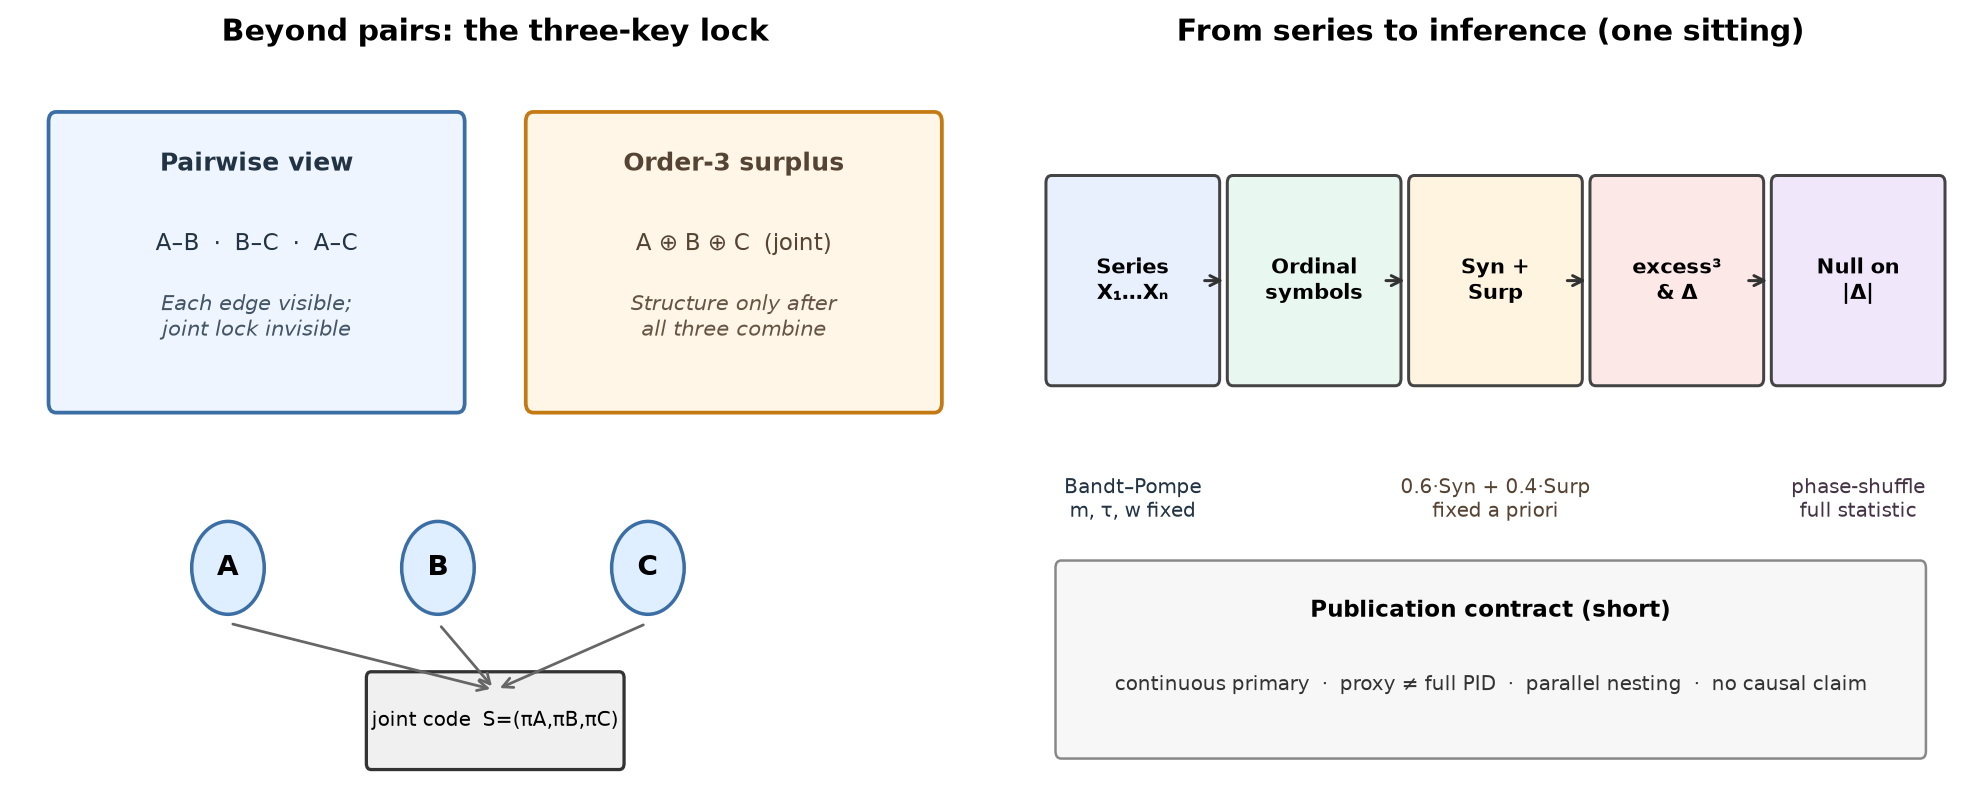
\includegraphics[width=0.98\textwidth]{figures/fig_pedagogical_overview.png}
\caption{Pedagogical overview for first contact. \textbf{Left:} pairwise
edges can look fine while a joint ``three-key'' code is invisible until all
channels are read together. \textbf{Right:} pipeline from series to
inference under the fixed contract (ordinal encoding, hybrid score, null on
the full $|\Delta|$). This figure is teaching material; equations and the
G0--G3 battery live in the methods paper \citep{Padilla2026excess3}.}
\label{fig:pedagogical}
\end{figure}

\subsection{What we deliberately do not do here}

\begin{itemize}[leftmargin=*,itemsep=2pt]
  \item We do \textbf{not} re-derive the full RECD / Systemic Tau framework.
  \item We do \textbf{not} dump every synthetic figure and hyperparameter
  table from the methods paper.
  \item We do \textbf{not} claim that excess$^3$ is ``emergence proved'' or
  ``causation found''.
  \item We do \textbf{not} lower the scientific standard of the methods
  paper; we raise the accessibility of the \emph{ideas} behind it.
\end{itemize}

% =============================================
\section{The core idea in one sitting}
\label{sec:core}

\subsection{A three-variable lock}

Imagine three binary indicators from a monitoring system:
\begin{center}
$A$ = rainfall high? \quad
$B$ = mosquito density high? \quad
$C$ = fever cases high?
\end{center}
You might find:
\begin{itemize}[leftmargin=*,itemsep=2pt]
  \item $A$ alone is only weakly related to $C$;
  \item $B$ alone is only weakly related to $C$;
  \item $A$ and $B$ together tightly constrain $C$.
\end{itemize}
In everyday language: \emph{the combination carries something the pairs do
not}. In information language: there is \textbf{order-3 synergistic
structure} (or synergistic surplus).

A related but different pattern is the opposite: $A$, $B$, and $C$ all rise
and fall together because of one shared driver (temperature, seasonality, a
common shock). Then pairs already explain most of the joint behaviour. That
is more like \textbf{redundancy} or common-cause locking than pure
order-3 synergy.

\begin{keyidea}
High-order dependence is about \textbf{organisation among variables}, not
about whether any single variable has large variance. A quiet system can
still reorganise its joint code; a noisy system can look ``active'' without
true multi-variable structure.
\end{keyidea}

\subsection{What excess$^3$ tries to answer}

excess$^3$ is an operational answer to a narrow question:

\begin{quote}
\emph{In a sliding window of multivariate observations (after a symbolic
encoding), how much joint surplus remains after we account for pairwise
structure and for simple independence?}
\end{quote}

It returns a non-negative continuous score over time. Larger values mean
more of that surplus under the chosen encoding and window. Contrasts
$\Delta\mathrm{excess3}$ (before vs after an event; condition A vs B) are
usually more scientifically useful than absolute levels.

\subsection{The one-line formula (preview)}

You will understand every term by Section~\ref{sec:build}. For orientation
only:
\begin{equation}
\label{eq:preview}
\mathrm{excess3}
=
0.6\,\mathrm{Syn}
+
0.4\,\mathrm{Surp}.
\end{equation}
\begin{itemize}[leftmargin=*,itemsep=2pt]
  \item $\mathrm{Syn}$ = residual multi-information after subtracting a
  pairwise baseline (``what pairs do not explain'').
  \item $\mathrm{Surp}$ = how much more often joint symbol combinations
  occur than under full independence.
  \item The weights $0.6$ and $0.4$ are \textbf{fixed in advance}. They are
  not optimised on your scientific dataset.
\end{itemize}

\begin{warningbox}
If you re-tune the weights on the same data you later claim results from,
you have turned a pre-specified test statistic into a flexible descriptor.
That may still be exploratory---but it is no longer the same methodological
object.
\end{warningbox}

% =============================================
\section{Analogies that carry the mathematics}
\label{sec:analogies}

Formal definitions come later. First, three analogies that map cleanly onto
what the measure does.

\subsection{The safe with two keys vs three keys}

\begin{itemize}[leftmargin=*,itemsep=3pt]
  \item \textbf{Pairwise world:} any two keys open something useful.
  Looking at pairs is enough.
  \item \textbf{Order-3 synergistic world:} the vault opens only when three
  keys are combined in the right pattern. Any pair looks uninformative;
  the triple is decisive.
  \item \textbf{Common-driver world:} one master key turns all locks. Pairs
  look extremely informative; the ``extra'' from the triple is small once
  pairs are accounted for.
\end{itemize}
excess$^3$ is closer to detecting the \emph{three-key} situation, while
still remaining sensitive to some joint surprises that pure pair-subtraction
might underplay (that is why it has two ingredients).

\subsection{Orchestra vs soloists}

If each instrument plays louder, univariate early-warning tools may fire.
If the instruments start coordinating in a new ensemble pattern---without
any soloist becoming extreme---you need a relational measure. excess$^3$ is
one way to listen for \emph{ensemble code} among three or more parts.

\subsection{Password vs checksum}

A password that is the XOR of two other bits is a classic synergy toy: each
bit alone is noise; together they determine the third. A checksum that
merely copies a shared flag is redundancy. Section~\ref{sec:xor} calculates
the password case by hand.

\begin{fieldbox}
\textbf{Ecology.} Species A and B may each correlate weakly with a collapse
indicator $C$, yet the combination ``A low and B high'' may lock $C$.\\
\textbf{Physiology.} Heart-rate, respiration, and blood-pressure patterns
may reorganise jointly before any channel crosses a clinical threshold.\\
\textbf{Climate.} Three regional indices can reorganise their co-occurrence
code near a regime shift even if pairwise correlations change only mildly.
\end{fieldbox}

% =============================================
\section{Why pairs are not enough}
\label{sec:pairs}

\subsection{What pairwise tools already give you}

Scientists already use excellent pairwise tools:
\begin{itemize}[leftmargin=*,itemsep=2pt]
  \item Pearson / Spearman correlations;
  \item mutual information $I(X;Y)$;
  \item transfer entropy and Granger-style directed tests;
  \item network edges based on significant pairs.
\end{itemize}
These answer: \emph{how are two variables related?} They do not fully
answer: \emph{is there structure that only appears when three or more are
considered jointly?}

\subsection{A minimal counterexample (XOR intuition)}

Suppose three binary variables satisfy $C = A \oplus B$ (XOR), with $A$ and
$B$ fair coins. Then:
\begin{itemize}[leftmargin=*,itemsep=2pt]
  \item $I(A;C)=0$, $I(B;C)=0$, $I(A;B)=0$ (pairs look independent);
  \item but $(A,B)$ determines $C$ completely.
\end{itemize}
Any analysis that only draws a network of pairwise edges will conclude
``nothing is related.'' A high-order lens sees a tight joint law.

\begin{keyidea}
Pairwise null results do \textbf{not} imply ``no dependence in the
system.'' They imply ``no dependence visible at order~2 under this
estimator.''
\end{keyidea}

\subsection{The opposite trap: calling every triple ``synergy''}

Not every interesting three-variable pattern is synergistic surplus. Shared
seasonality, one latent shock, or a strong common driver can make all pairs
light up. That is scientifically important---but it is a different geometry.
excess$^3$ tries to emphasise residual joint structure after a pairwise
baseline, plus independence surprise. It is still a \textbf{proxy}, not a
court verdict that ``true synergy exists in nature.''

% =============================================
\section{A gentle information primer}
\label{sec:primer}

This section is intentionally elementary. Skip it if entropy and mutual
information are already fluent for you; otherwise it is the bridge into
Section~\ref{sec:build}.

\subsection{Uncertainty as a number: entropy}

\begin{defbox}
\textbf{Entropy} $H(X)$ measures how unpredictable a variable is under a
chosen unit (here: bits). A fair coin has $H=1$~bit. A coin that always
lands heads has $H=0$.
\end{defbox}

For a discrete variable with probabilities $p(x)$,
\begin{equation}
H(X)=-\sum_x p(x)\log_2 p(x).
\end{equation}
You do not need deep measure theory to use this: plug in frequencies from a
window of symbols.

\subsection{Shared information: mutual information}

\begin{defbox}
\textbf{Mutual information} $I(X;Y)$ measures how much knowing $X$ reduces
uncertainty about $Y$ (and vice versa). It is zero when $X$ and $Y$ are
independent under the estimated distribution.
\end{defbox}

\begin{equation}
I(X;Y)=H(X)+H(Y)-H(X,Y).
\end{equation}
Interpretation checklist:
\begin{itemize}[leftmargin=*,itemsep=2pt]
  \item $I=0$: no detectable pairwise dependence (under this estimator);
  \item larger $I$: stronger pairwise dependence;
  \item $I$ is symmetric and non-negative (for the usual Shannon version).
\end{itemize}

\subsection{More than two variables: total correlation}

\begin{defbox}
\textbf{Total correlation} (multiinformation)
\[
\mathrm{TC}(X_1,\ldots,X_N)
=
\sum_{i=1}^{N}H(X_i)-H(X_1,\ldots,X_N)
\]
measures \emph{total} shared information among $N$ variables. It is zero
only under full mutual independence.
\end{defbox}

TC is large when the joint is far more organised than the product of
marginals. Crucially, TC does \textbf{not} by itself tell you whether that
organisation is mostly pairs or mostly higher-order structure.

\subsection{The missing piece: a pairwise baseline}

To isolate something more like ``beyond pairs,'' subtract a baseline built
from pairwise mutual informations. In the excess$^3$ construction the
baseline is scaled mean pairwise MI:
\begin{equation}
I_{\mathrm{pair}}
=
(N-1)\cdot
\overline{I}_{ij},
\end{equation}
where $\overline{I}_{ij}$ is the average of $I(X_i;X_j)$ over pairs. The
factor $(N-1)$ puts the baseline on a scale comparable to TC
\citep{Padilla2026framework,Padilla2026excess3}.

Then
\begin{equation}
\mathrm{Syn}
=
\bigl[\mathrm{TC}-I_{\mathrm{pair}}\bigr]_+
=
\max\{\mathrm{TC}-I_{\mathrm{pair}},0\}.
\end{equation}
If pairs already explain the multiinformation, $\mathrm{Syn}$ collapses
toward zero. If multiinformation outruns the pairwise baseline,
$\mathrm{Syn}$ rises.

\begin{warningbox}
$\mathrm{Syn}$ is a \textbf{residual construction}, not a mystical proof of
emergence. Different baselines yield different residuals. The methods paper
fixes one baseline aligned with the reference software.
\end{warningbox}

\subsection{Independence surprise}

Even after residual multiinformation, it helps to ask a second question:
\begin{quote}
\emph{Do particular joint combinations occur more often than the product of
marginals would allow?}
\end{quote}
That is $\mathrm{Surp}$: a weighted sum of positive log-ratio surprises for
joint symbol tuples. It is complementary to $\mathrm{Syn}$:
\begin{itemize}[leftmargin=*,itemsep=2pt]
  \item $\mathrm{Syn}$ lives in multiinformation-minus-pairs geometry;
  \item $\mathrm{Surp}$ lives in ``joint co-occurrence vs independence''
  geometry.
\end{itemize}

% =============================================
\section{From raw series to symbols (why ordinal encoding?)}
\label{sec:symbols}

\subsection{The practical problem}

Real variables have different units, drifts, and heavy tails. Direct
plug-in entropies on raw continuous values need binning choices that can
dominate the result.

\subsection{Bandt--Pompe ordinal patterns in one paragraph}

Bandt--Pompe encoding replaces a local segment of a series by the
\textbf{rank pattern} of its values \citep{BandtPompe2002}. For embedding
dimension $m=3$, each window of three samples becomes one of $3!=6$
possible order patterns (``up-up'', ``peak'', ``trough'', etc.).

Why scientists like this:
\begin{itemize}[leftmargin=*,itemsep=2pt]
  \item invariant to monotone transformations of each channel;
  \item focuses on relational shape rather than absolute amplitude;
  \item yields a discrete alphabet where information quantities are
  straightforward to estimate in short windows.
\end{itemize}

\begin{keyidea}
excess$^3$ as used in RECD is typically computed on \textbf{ordinal symbol
streams}, not on raw millimetres of mercury or raw case counts. That is a
feature for cross-domain comparison, and a limitation if your scientific
claim is about amplitudes rather than order patterns.
\end{keyidea}

\subsection{Windows}

Everything is estimated inside a sliding window of length $w$ (reference
software often uses $w=13$ with $m=3$). Think of excess$^3(t)$ as a local
``joint organisation score'' ending at time $t$, not as a single number for
the whole study.

% =============================================
\section{Building excess$^3$ brick by brick}
\label{sec:build}

\subsection{The pipeline}

\begin{enumerate}[leftmargin=*,itemsep=3pt]
  \item Start with $N$ aligned time series (the interesting scientific case
  is $N=3$, but the formulas extend).
  \item Encode each series into ordinal symbols.
  \item In a window, estimate entropies of each channel, all pairs, and the
  full joint.
  \item Compute $\mathrm{TC}$, $I_{\mathrm{pair}}$, $\mathrm{Syn}$,
  $\mathrm{Surp}$.
  \item Combine: $\mathrm{excess3}=0.6\,\mathrm{Syn}+0.4\,\mathrm{Surp}$.
  \item Optionally threshold: $\Phi_3=\mathbf{1}\{\mathrm{excess3}>\theta_3\}$.
\end{enumerate}

\subsection{Component table}

\begin{table}[H]
\centering
\caption{The moving parts of excess$^3$ in plain language.}
\label{tab:parts}
\small
\begin{tabularx}{\textwidth}{@{}>{\raggedright\arraybackslash}p{2.6cm} X X@{}}
\toprule
\textbf{Symbol} & \textbf{Plain meaning} & \textbf{If it is high\ldots} \\
\midrule
TC
  & Total shared information among the $N$ symbol streams
  & The joint is organised far beyond independence \\
$I_{\mathrm{pair}}$
  & Pairwise baseline (scaled mean pairwise MI)
  & Pairs already carry a lot of structure \\
Syn
  & $\max(\mathrm{TC}-I_{\mathrm{pair}},0)$
  & Multiinformation exceeds what pairs explain \\
Surp
  & Positive surprise of joints vs product of marginals
  & Specific joint combinations are over-represented \\
excess$^3$
  & $0.6\,\mathrm{Syn}+0.4\,\mathrm{Surp}$
  & Hybrid synergistic surplus (continuous) \\
$\Phi_3$
  & Binary tick if excess$^3>\theta_3$
  & Only a discretisation for counts/displays \\
\bottomrule
\end{tabularx}
\end{table}

\subsection{Why a hybrid?}

A single pure atom from a full PID lattice is conceptually cleaner---and
often statistically harder at the sample sizes of ecology, epidemiology, or
field physiology. The hybrid is a deliberate engineering choice:
\begin{itemize}[leftmargin=*,itemsep=2pt]
  \item $\mathrm{Syn}$ pushes against ``pairs already explained it'';
  \item $\mathrm{Surp}$ keeps sensitivity to joint co-occurrence structure;
  \item fixed weights keep the object pre-specified and comparable across
  studies.
\end{itemize}

This is why the methods paper calls excess$^3$ a \textbf{computable proxy}
rather than ``the'' synergy atom \citep{Padilla2026excess3}.

% =============================================
\section{Worked example: the XOR-like window}
\label{sec:xor}

This is the pedagogical heart of the guide. Numbers are tiny on purpose.

\begin{workbox}
\textbf{Setup.} Window length $w=8$, three symbol streams with alphabet
$\{0,1\}$. The eight rows implement a password-like lock: each pair is
uninformative, but the triple is tightly constrained (XOR geometry).
\end{workbox}

\begin{equation*}
\begin{array}{c@{\;\;}c@{\;\;}c@{\qquad}l}
\pi^{(1)} & \pi^{(2)} & \pi^{(3)} & \\
\hline
0 & 0 & 0 & \\
0 & 1 & 1 & \\
1 & 0 & 1 & \\
1 & 1 & 0 & \text{each of these four joint types appears twice} \\
0 & 0 & 0 & \\
0 & 1 & 1 & \\
1 & 0 & 1 & \\
1 & 1 & 0 &
\end{array}
\end{equation*}

\paragraph{Step 1 --- single-channel entropies.}
Each channel is half $0$s and half $1$s, so $H(\pi^{(i)})=1$ bit.

\paragraph{Step 2 --- joint entropy.}
There are four joint types, each with probability $1/4$, so the joint
entropy is $H(\pi^{(1:3)})=2$ bits.

\paragraph{Step 3 --- total correlation.}
\begin{equation*}
\mathrm{TC}
=
(1+1+1)-2
=
1.
\end{equation*}

\paragraph{Step 4 --- pairwise baseline.}
Every pair is balanced in a way that pairwise MI vanishes, so
$\overline{I}_{ij}=0$ and $I_{\mathrm{pair}}=0$.

\paragraph{Step 5 --- Syn.}
\begin{equation*}
\mathrm{Syn}
=
[1-0]_+
=
1.
\end{equation*}

\paragraph{Step 6 --- Surp.}
Under independence, each joint triple would have probability
$(1/2)^3=1/8$. Empirically each observed type has probability $1/4$. The
log-ratio is
\begin{equation*}
\log_2\frac{1/4}{1/8}=1,
\end{equation*}
and four types each contribute $(1/4)\cdot 1$, so $\mathrm{Surp}=1$.

\paragraph{Step 7 --- excess$^3$.}
\begin{equation*}
\mathrm{excess3}
=
0.6\cdot 1 + 0.4\cdot 1
=
1.0.
\end{equation*}

\begin{keyidea}
In the XOR window, \textbf{both} ingredients fire. Pairs see nothing; the
joint sees everything. That is the pedagogical prototype of order-3
synergistic surplus.
\end{keyidea}

\subsection{Contrast: pure common driver}

If all three channels are identical (only joints like $(0,0,0)$ and
$(1,1,1)$ appear), pairs become extremely informative. Then
$I_{\mathrm{pair}}$ can absorb most of TC, so $\mathrm{Syn}\to 0$, while
$\mathrm{Surp}$ may remain large because the joint is still far from
independence. excess$^3$ then lives mainly on the surprise leg. This is
intentional: redundant locking and XOR-like locking are different geometries
\citep{Padilla2026excess3}.

% =============================================
\section{How to read magnitudes and signs}
\label{sec:read}

\subsection{Absolute level vs contrast}

\begin{table}[H]
\centering
\caption{Reading excess$^3$ values without overclaiming.}
\label{tab:reading}
\small
\begin{tabularx}{\textwidth}{@{}>{\raggedright\arraybackslash}p{3.4cm} X@{}}
\toprule
\textbf{Pattern} & \textbf{Honest reading} \\
\midrule
excess$^3(t)\approx 0$
  & Joint structure is largely explainable by pairs or independence under
    this encoding and window. \\
Sustained elevation
  (often $\gtrsim 0.10$--$0.20$, domain-dependent)
  & Suggests detectable synergistic surplus---not a universal clinical
    cut-off. \\
$\Delta\mathrm{excess3}$ pre/post
  & Usually the scientific object of interest (did organisation change?). \\
Negative $\Delta$ after a reorganisation
  & Possible and informative: stronger common coupling can inflate pairwise
    baselines and shrink residual Syn. \\
Binary $\Phi_3$ alone
  & Incomplete if continuous curves are ignored; thresholds can saturate. \\
\bottomrule
\end{tabularx}
\end{table}

\begin{warningbox}
There is \textbf{no universal threshold} that means ``synergy happened''
across ecology, cardiology, and climate. Always interpret with a null
(Section~\ref{sec:nulls}) and report encoding parameters $(m,\tau,w)$.
\end{warningbox}

\subsection{Why a change can be negative even when ``something real happened''}

This is one of the most important practical lessons from synthetic
validation \citep{Padilla2026excess3}. In a shared-latent generator, when
common coupling strengthens after an event, pairwise mutual informations
rise. Because $\mathrm{Syn}$ subtracts a pairwise baseline, residual
multiinformation can \emph{fall} even though the system truly reorganised.

Therefore inference is performed on
$|\Delta\mathrm{excess3}|$
(two-sided extremity under surrogates), not on a forced positive sign.

\begin{keyidea}
A negative $\Delta\mathrm{excess3}$ is not automatically a failed
experiment. It can mean: \textbf{pairwise structure absorbed the change}.
Report the sign, explain it, and test extremity against a null.
\end{keyidea}

\subsection{Continuous primacy}

The binary indicator
\begin{equation}
\Phi_3(t)=\mathbf{1}\{\mathrm{excess3}(t)>\theta_3\}
\end{equation}
is useful for tick counts and raster-like displays. It is a
\textbf{secondary} discretisation. Continuous excess$^3$ and
$\Delta\mathrm{excess3}$ are primary for scientific contrasts. In synthetic
batteries, a low reference $\theta_3$ can saturate occupancy while continuous
$\Delta$ still discriminates arms \citep{Padilla2026excess3}.

% =============================================
\section{What excess$^3$ is not}
\label{sec:not}

This section exists to protect your reputation in interdisciplinary review.

\begin{enumerate}[leftmargin=*,itemsep=4pt]
  \item \textbf{Not causation.}
  Co-occurrence beyond pairs is not a directed mechanism. Causal claims
  need design, lags, interventions, or explicit causal models.

  \item \textbf{Not a full PID synergy atom.}
  PID isolates unique, redundant, and synergistic atoms on a lattice
  \citep{Williams2010,Bertschinger2014}. excess$^3$ is a practical proxy in
  that neighbourhood, not a replacement theorem.

  \item \textbf{Not proof of strong emergence.}
  ``Irreducible in this statistical sense'' is weaker than metaphysical
  emergence. Keep the language operational.

  \item \textbf{Not a free lunch for tiny samples.}
  Joint symbol distributions need enough window mass. Short $T$, large $N$,
  or large alphabets inflate variance and bias.

  \item \textbf{Not interchangeable with O-information without care.}
  O-/S-information provide global redundancy-vs-synergy decompositions
  \citep{Rosas2019}. They are relatives, not synonyms.

  \item \textbf{Not ``whatever the weights say after tuning.''}
  Pre-specification is part of the object. If you retune, say so and treat
  claims as exploratory.
\end{enumerate}

\begin{table}[H]
\centering
\caption{Positioning for non-specialists: what family of questions each
tool answers.}
\label{tab:position}
\small
\begin{tabularx}{\textwidth}{@{}>{\raggedright\arraybackslash}p{3.0cm}
  >{\raggedright\arraybackslash}X
  >{\raggedright\arraybackslash}p{2.0cm}
  >{\raggedright\arraybackslash}X@{}}
\toprule
\textbf{Measure} & \textbf{Main question} & \textbf{Cost} &
\textbf{Relation to excess$^3$} \\
\midrule
Interaction information
  & Signed three-variable interaction (can be negative)
  & Low
  & Conceptual cousin; not identical \\
O-information
  & Global redundancy vs synergy balance
  & Medium
  & More global; not locked to order exactly 3 \\
PID synergy atom
  & Pure synergistic atom on the lattice
  & High
  & Conceptual target; often hard to estimate \\
\textbf{excess$^3$}
  & Pre-specified hybrid order-3 surplus proxy
  & Low--med.
  & This guide's object \\
\bottomrule
\end{tabularx}
\end{table}

% =============================================
\section{How inference works (without the full methods appendix)}
\label{sec:nulls}

\subsection{The question a null must answer}

You observed $\Delta\mathrm{excess3}$ between two regimes. Could a process
with similar single-channel spectra but destroyed cross-variable phase
relationships produce a $\Delta$ at least as extreme?

\subsection{Phase-shuffle in plain language}

A practical surrogate:
\begin{enumerate}[leftmargin=*,itemsep=2pt]
  \item Fourier-transform each channel;
  \item randomise phases (preserving power spectrum, roughly);
  \item invert, re-encode ordinal symbols, recompute excess$^3$ and
  $\Delta$;
  \item repeat $B$ times to build a null distribution;
  \item place the observed $|\Delta|$ in that distribution.
\end{enumerate}
This breaks fine-grained cross-channel organisation while retaining much of
each channel's autocorrelation structure---a better straw man than pure
white noise for many time-series settings
\citep{Schreiber2000,Padilla2026excess3}.

\begin{warningbox}
Do not only compare ``mean of observed windows vs mean of null means''
without ranking the \textbf{full statistic} you care about. The methods
paper emphasises testing $\Delta\mathrm{excess3}$ (or the chosen contrast)
against the surrogate distribution of that same contrast.
\end{warningbox}

\subsection{What synthetic validation taught us (selected)}

Under a controlled battery (near-null independent AR channels; planted
shared-latent reorganisation; coupled logistics; pure pairwise control), the
methods paper finds, in short:
\begin{itemize}[leftmargin=*,itemsep=2pt]
  \item near-null arms stay near zero $\Delta$ with non-extreme surrogate
  $p$-values;
  \item planted joint reorganisation yields extreme $|\Delta|$ at high rates;
  \item the sign under shared-latent strengthening can be negative;
  \item continuous $\Delta$ discriminates even when binary occupancy
  saturates at a low threshold.
\end{itemize}
Those results justify careful use; they do \textbf{not} license universal
thresholds on real observational data. See
\citep{Padilla2026excess3} for numbers, figures, and claim gates.

% =============================================
\section{A minimal path into Systemic Tau / RECD}
\label{sec:recd_min}

You can use excess$^3$ as a standalone high-order feature. In the broader
programme it is Level~3 of a nested ordinal hierarchy
\citep{Padilla2026framework}:

\begin{itemize}[leftmargin=*,itemsep=3pt]
  \item \textbf{Systemic Tau} ($\tau_s$): a continuous ``thermometer'' of
  multivariate rank concordance (relational coherence).
  \item \textbf{RECD}: a discrete intrinsic clock advanced by ordinal
  conjunctions at several depths.
  \item \textbf{Level 1 ($\Phi_1$):} coincidence-like events.
  \item \textbf{Level 2 ($\Phi_2$):} persistent pairwise relational events.
  \item \textbf{Level 3:} synergistic surplus---continuous excess$^3$ and
  optional binary $\Phi_3$.
\end{itemize}

\paragraph{Operative nesting (important).}
It is tempting to imagine a logical tower
$\Phi_1\Rightarrow\Phi_2\Rightarrow\Phi_3$.
In the reference construction the levels are computed \textbf{in parallel}.
Order-3 irreducibility is statistical (via the excess construction), not a
hard Boolean implication. This is design decision~6 in
Section~\ref{sec:design}.

\begin{keyidea}
If you only need a high-order dependence feature for a classifier or an
early-warning panel, you can start with excess$^3$ alone. If you need the
full Kairos-style clock narrative, read the framework paper after this
guide---not before.
\end{keyidea}

% =============================================
\section{Field vignettes: how to talk about it in your domain}
\label{sec:fields}

These vignettes are \textbf{framing aids}, not empirical claims about
particular datasets.

\subsection{Ecology and conservation}

\begin{fieldbox}
\textbf{Question.} Do three indicators of ecosystem state reorganise their
joint ordinal code before a regime shift, even if no single indicator has
crossed a classical early-warning threshold?
\end{fieldbox}
Pair with classical variance / lag-1 autocorrelation tools
\citep{Scheffer2009,Dakos2012}. Report excess$^3$ as a relational complement,
not a replacement. Watch for seasonality as a common driver that can inflate
pairs.
\par\noindent\textit{Allowed:} ``joint ordinal reorganisation beyond pairs.''
\textit{Forbidden:} ``proved ecosystem emergence / tipping caused by synergy.''

\subsection{Epidemiology and environmental health}

\begin{fieldbox}
\textbf{Question.} Do climate, vector, and incidence symbols develop
beyond-pairwise co-occurrence structure around outbreak onsets?
\end{fieldbox}
Be explicit: excess$^3$ does not identify which variable ``causes'' cases.
It flags joint reorganisation worth mechanistic follow-up.
\par\noindent\textit{Allowed:} ``beyond-pairwise co-occurrence around onset.''
\textit{Forbidden:} ``climate caused incidence via excess$^3$.''

\subsection{Physiology and critical care}

\begin{fieldbox}
\textbf{Question.} Do cardiorespiratory ordinal patterns show synergistic
surplus changes around decompensation windows?
\end{fieldbox}
Continuous primacy matters: binary alarms may sit silent while continuous
excess$^3$ drifts. Thresholds must be justified in-domain, never copied
blindly from software defaults.
\par\noindent\textit{Allowed:} ``continuous surplus drift under a pre-specified null.''
\textit{Forbidden:} ``$\Phi_3$ alarm proves decompensation.''

\subsection{Climate and Earth system science}

\begin{fieldbox}
\textbf{Question.} Near a potential tipping element, do three regional
indices show residual joint structure beyond pairwise teleconnection maps?
\end{fieldbox}
Compare against phase-shuffle nulls that preserve much of each index's
spectrum. Document encoding $(m,\tau,w)$ as carefully as a filter choice.
\par\noindent\textit{Allowed:} residual joint structure vs pairwise maps.
\textit{Forbidden:} ``tipping confirmed by synergy score alone.''

\subsection{Neuroscience and cognitive science}

\begin{fieldbox}
\textbf{Question.} Is there order-3 synergistic surplus among three neural
or behavioural readouts during integration epochs?
\end{fieldbox}
Readers in this field often expect PID language. State clearly that
excess$^3$ is a proxy neighbour of synergy atoms, not a lattice decomposition
\citep{Williams2010,Rosas2019}.
\par\noindent\textit{Allowed:} ``proxy for order-3 surplus (not a PID atom).''
\textit{Forbidden:} ``we measured the synergy atom of consciousness.''

\subsection{Social and economic systems}

\begin{fieldbox}
\textbf{Question.} Do three market or mobility series reorganise jointly
around shocks in a way edge-networks miss?
\end{fieldbox}
Common shocks are the main confounder. Negative $\Delta$ after
synchronisation spikes is a live possibility; interpret with the pairwise
baseline story.
\par\noindent\textit{Allowed:} ``joint reorganisation; possible pairwise absorption.''
\textit{Forbidden:} ``markets lost integration because $\Delta<0$.''

% =============================================
\section{A first-analysis workflow}
\label{sec:workflow}

\begin{enumerate}[leftmargin=*,itemsep=4pt]
  \item \textbf{State the scientific contrast} before computing.
  Pre/post event? Treatment vs control? Seasonal baseline vs anomaly?

  \item \textbf{Choose $N=3$ channels} with a joint hypothesis (not three
  random leftover sensors).

  \item \textbf{Fix encoding parameters a priori:} $m$, $\tau$, $w$,
  stride. Write them down before looking at $p$-values.

  \item \textbf{Compute continuous excess$^3(t)$} and the pre-specified
  contrast $\Delta$.

  \item \textbf{Run phase-shuffle (or design-based) nulls} on that same
  contrast; report median $p$ and fraction extreme if using ensembles.

  \item \textbf{Report Syn and Surp separately} at least in a supplement:
  which leg moved?

  \item \textbf{Show continuous curves}; treat $\Phi_3$ as secondary.

  \item \textbf{Language audit:} dependence/organisation/surplus---not
  causation/emergence proved.

  \item \textbf{Sensitivity:} at least one alternate window length or $m$
  if sample size allows.

  \item \textbf{Point to the methods paper} for estimator details and
  software alignment.
\end{enumerate}

\subsection{Minimum reporting checklist (copy into lab notes)}

\begin{itemize}[leftmargin=*,itemsep=2pt]
  \item Series length $T$, number of channels $N$, sampling rate;
  \item Bandt--Pompe $(m,\tau)$, window $w$, stride;
  \item weights $(0.6,0.4)$ and statement that they were not tuned on this
  dataset;
  \item primary statistic: continuous excess$^3$ / $\Delta\mathrm{excess3}$;
  \item $\theta_3$ only if $\Phi_3$ is used, with saturation checks;
  \item null model, $B$, two-sided vs one-sided rule;
  \item software commit / version when available;
  \item explicit non-claims (not causal, not full PID).
\end{itemize}

% =============================================
\section{Six design decisions (the fixed contract)}
\label{sec:design}

When readers first meet excess$^3$, six questions almost always reappear.
The short answers below are the \textbf{methodological contract} shared with
the methods paper \citep{Padilla2026excess3}: they are design choices, not
optional footnotes. If you remember nothing else from this guide's middle
chapters, remember these six.

\paragraph{1.\ Why $0.6/0.4$?}
The weights
$(\alpha_{\mathrm{Syn}},\alpha_{\mathrm{Surp}})=(0.6,0.4)$ are
\textbf{heuristic constants fixed a~priori}. They lean slightly toward the
residual multiinformation leg (Syn) over independence surprise (Surp), but
they are \emph{not} fitted by cross-validation, grid search, or any other
optimiser on the scientific dataset under test. That pre-specification
protects \emph{falsifiability}: excess$^3$ stays a declared statistic rather
than a dial you turn until a favourite $p$-value appears. You may pre-register
a different pair \emph{before} looking at the hypothesis data; silent
re-weighting on the claim dataset is not compatible with presenting the
canonical excess$^3$ object.

\paragraph{2.\ Syn versus Surp.}
$\mathrm{Syn}=[\mathrm{TC}-I_{\mathrm{pair}}]_+$ asks: after we
\textbf{subtract} a pairwise mutual-information baseline from total
correlation, how much multiinformational organisation remains?
$\mathrm{Surp}$ asks a different question: which joint symbol tuples are
\textbf{more frequent than under complete independence}
($p_{\mathrm{obs}}$ vs.\ $\prod_i p_i$), counting only positive log-ratio
contributions? The hybrid keeps both lenses visible. XOR-like locks tend to
light both; pure common-driver locking often collapses Syn while Surp stays
large (Section~\ref{sec:xor}).

\paragraph{3.\ excess$^3$ versus $\Phi_3$.}
Continuous $\mathrm{excess3}(t)$ is the \textbf{primary} Level-3 readout:
trajectories, gradients, and contrasts $\Delta\mathrm{excess3}$ live on the
continuous scale. Binary
$\Phi_3=\mathbf{1}\{\mathrm{excess3}>\theta_3\}$ exists only for tick
counts, raster-like displays, and rate summaries. If $\theta_3$ sits below
the bulk of the continuous distribution, $\Phi_3$ occupancy can saturate
even when $\Delta$ still separates regimes---that is a threshold issue, not
proof that ``Level~3 did nothing'' (Section~\ref{sec:read}).

\paragraph{4.\ Not a complete PID.}
excess$^3$ is a \textbf{computable proxy} for order-3 synergistic surplus,
not a full partial information decomposition. It does not isolate unique,
redundant, and synergistic atoms of a PID lattice
\citep{Williams2010,Bertschinger2014}. The natural theoretical extension is
to replace the hybrid formula by a stable PID synergy atom when sample size
and estimator quality allow; until then, the hybrid is the operational
contract (Section~\ref{sec:not}).

\paragraph{5.\ The null.}
Inference targets the \textbf{full declared contrast}---usually
$|\Delta\mathrm{excess3}|$ under a two-sided Monte Carlo rule---not a vague
``mean vs mean of means.'' The default surrogate is independent
phase-shuffle (or any pre-specified alternative that preserves relevant
univariate structure while \textbf{breaking cross-channel dependence}).
Ranking the observed contrast inside the surrogate cloud is the protocol;
mean-versus-mean alone is an anti-pattern (Section~\ref{sec:nulls}).

\paragraph{6.\ Operative nesting.}
In RECD language one may speak of deeper levels as stronger claims. In
software, $\Phi_1$, $\Phi_2$, and excess$^3$/$\Phi_3$ are computed
\textbf{in parallel} from the same symbolic window. There is no hard
Boolean implication $\Phi_1\Rightarrow\Phi_2\Rightarrow\Phi_3$ in the
reference code. Order-3 irreducibility is inferred \emph{statistically}
through the excess construction (Syn after the pairwise baseline, plus
Surp), not by forcing a chain of logical gates
(Section~\ref{sec:recd_min}).

\begin{keyidea}
Weights fixed before the claim data; Syn subtracts pairs, Surp scores
over-represented joints; continuous first, binary only for ticks; proxy not
full PID; nulls on full $\Delta$; RECD levels in parallel, not a Boolean
ladder. That is the whole design contract in one breath.
\end{keyidea}

% =============================================
\section{Common misconceptions (FAQ)}
\label{sec:faq}

Section~\ref{sec:design} already settles the six design decisions. The
questions below cover remaining confusions that still show up in seminars
and reviews.

\paragraph{Q1. Is excess$^3$ just ``the synergy from PID''?}
No---see also design decision~4. It is a hybrid proxy for stable
pre-specified use when full PID estimation is fragile or unnecessary for
the claim.

\paragraph{Q2. If excess$^3$ is high, did we find emergence?}
You found elevated residual joint organisation under a specific encoding.
That can support an emergence-\emph{related} discussion; it does not settle
philosophical emergence.

\paragraph{Q3. Why not always use interaction information alone?}
Interaction information is a valuable cousin and can be negative
\citep{McGill1954,Timme2018}. excess$^3$ is a different operational object:
non-negative hybrid residual plus independence surprise, with fixed weights
and a software-aligned pipeline.

\paragraph{Q4. My $\Delta$ is negative but the system clearly changed. Failed?}
Not necessarily. Check whether pairwise dependence exploded. Look at
Syn vs Surp separately. Test $|\Delta|$ against surrogates.

\paragraph{Q5. Can I optimise the $0.6/0.4$ weights with cross-validation?}
You can explore weight sensitivity in a methods supplement. If weights are
chosen to maximise your scientific effect on the same data, label the
analysis exploratory and do not present it as the pre-specified excess$^3$
statistic (design decision~1).

\paragraph{Q6. Do I need the full RECD story to publish with excess$^3$?}
No. You need honest definition, nulls, and domain interpretation. RECD
context is optional framing (design decision~6: levels need not be a
Boolean tower).

\paragraph{Q7. Is binary $\Phi_3$ good enough for a paper?}
Usually not by itself. Continuous trajectories and contrasts should lead;
binary ticks can accompany them (design decision~3).

\paragraph{Q8. What sample size do I need?}
There is no universal $n$. Joint alphabets grow fast. Prefer longer series,
modest $m$, and surrogate tests. If the joint histogram is mostly empty,
you are not estimating high-order structure---you are estimating sparsity.

\paragraph{Q9. Can excess$^3$ replace early-warning indicators?}
No. Classical EWS tools remain powerful for many univariate bifurcation
routes \citep{Scheffer2009}. excess$^3$ is a relational complement.

\paragraph{Q10. Where is the code?}
Reference implementation lives in the Systemic Tau / RECD software stack
(\texttt{recd\_levels} / \texttt{\_synergy\_and\_surprise}); the methods
paper and its toy script document alignment
\citep{Padilla2026excess3,Padilla2026software}.

% =============================================
\section{A second worked sketch: reading a pre/post contrast}
\label{sec:delta_story}

Suppose a laboratory records three ordinalised channels around a known
perturbation at time $t^\star$. They compute:
\begin{center}
mean excess$^3$ before: $1.83$ \qquad
mean after: $1.73$ \qquad
$\Delta=-0.10$.
\end{center}
Phase-shuffle nulls put $|\Delta|$ in the extreme tail (e.g.\ median
$p\approx 0.01$ across realisations in a synthetic analogue).

\paragraph{Bad write-up.}
``Synergy decreased, therefore integration failed.''

\paragraph{Better write-up.}
``The pre-specified contrast $\Delta\mathrm{excess3}$ was negative and
surrogate-extreme. Separate inspection shows pairwise mutual information
increased after $t^\star$, shrinking the residual Syn term. We therefore
interpret the change as a reorganisation toward stronger common coupling
rather than as `nothing happened.' Continuous excess$^3$ remained the
primary readout; binary occupancy was saturated at the reference
threshold.''

This narrative mirrors lessons from the shared-latent synthetic arm without
requiring the reader to digest the full validation suite first
\citep{Padilla2026excess3}.

% =============================================
\section{Teaching notes (for courses and lab meetings)}
\label{sec:teaching}

\subsection{A 45-minute reading-group plan}

\begin{enumerate}[leftmargin=*,itemsep=2pt]
  \item 10 min: XOR intuition on the whiteboard (no software).
  \item 10 min: compute TC, Syn, Surp by hand from Section~\ref{sec:xor}.
  \item 10 min: discuss negative $\Delta$ and pairwise absorption.
  \item 10 min: domain vignette chosen by the group
  (Section~\ref{sec:fields}).
  \item 5 min: language audit (Section~\ref{sec:not}).
\end{enumerate}

\subsection{A half-day workshop plan}

\begin{enumerate}[leftmargin=*,itemsep=2pt]
  \item Morning: this guide through Section~\ref{sec:read}.
  \item Midday: run the public toy example script from the methods
  companion.
  \item Afternoon: each participant frames one contrast in their data
  (without $p$-hacking weights).
  \item Close: map open questions to the methods paper sections
  (nulls, estimation, limitations).
\end{enumerate}

\subsection{What to assign as required reading}

\begin{itemize}[leftmargin=*,itemsep=2pt]
  \item \textbf{Everyone:} this guide.
  \item \textbf{Implementers / methods reviewers:} methods paper
  \citep{Padilla2026excess3}.
  \item \textbf{Spanish-language groups:} dense introduction
  \citep{Padilla2026intro} (same contract and validation evidence).
  \item \textbf{Readers who need the full clock narrative:} framework
  paper \citep{Padilla2026framework}.
  \item \textbf{Optional classical background:} Bandt--Pompe
  \citep{BandtPompe2002}; early-warning review \citep{Scheffer2009}; PID
  entry points \citep{Williams2010,Timme2018}.
\end{itemize}

% =============================================
\section{Limitations (honest, still pedagogical)}
\label{sec:limits}

\begin{itemize}[leftmargin=*,itemsep=3pt]
  \item \textbf{Encoding dependence.} Ordinal patterns emphasise order, not
  amplitude. If your science is amplitude-first, say so and consider
  complementary measures.
  \item \textbf{Estimator dependence.} Plug-in entropies are transparent but
  biased in small samples. Changing estimators changes numeric scales.
  \item \textbf{Proxy gap.} Distance to a true PID synergy atom is not zero
  and is context-dependent.
  \item \textbf{Computational growth.} Moving from order 3 toward excess$^k$
  becomes expensive quickly.
  \item \textbf{Null mismatch.} Phase-shuffle is powerful, not universal. If
  your alternative hypothesis is a different kind of structure, design a
  matching null.
  \item \textbf{Interdisciplinary rhetoric risk.} Words like
  \emph{synergy}, \emph{emergence}, and \emph{integration} travel poorly
  across fields. Prefer operational phrasing in results sections.
\end{itemize}

% =============================================
\section{Where to go next}
\label{sec:next}

\begin{enumerate}[leftmargin=*,itemsep=3pt]
  \item \textbf{Methods companion.}
  Canonical equations, null protocol, synthetic G0--G3 validation, reporting
  checklist for manuscripts \citep{Padilla2026excess3}.

  \item \textbf{Spanish introduction.}
  Dense motivation and the full G0--G3 figure set in Spanish
  \citep{Padilla2026intro}.

  \item \textbf{Framework paper.}
  Systemic Tau as relational thermometer; RECD as intrinsic discrete time;
  how Level~3 sits in the paradigm \citep{Padilla2026framework}.

  \item \textbf{Software.}
  Reference implementation and reproducibility notes
  \citep{Padilla2026software}
  (\url{https://doi.org/10.5281/zenodo.20576241}).

  \item \textbf{Domain papers.}
  Apply the workflow of Section~\ref{sec:workflow} to your system; do not
  expect this guide to contain your field's empirical result.
\end{enumerate}

\begin{keyidea}
The highest-quality use of excess$^3$ is boring in the best sense:
pre-specified, continuous-first, null-tested, modest in language, and clear
about being a proxy for high-order dependence rather than a metaphysical
detector.
\end{keyidea}

% =============================================
\section{Glossary}
\label{sec:glossary}

\begin{description}[style=nextline,leftmargin=1.2em,itemsep=4pt]
  \item[Alphabet]
    The set of possible symbols after encoding (for Bandt--Pompe with
    embedding $m$, size $m!$).

  \item[Bandt--Pompe / ordinal pattern]
    Local rank-order encoding of a real-valued series
    \citep{BandtPompe2002}.

  \item[excess$^3$ / \texttt{excess3}]
    Hybrid continuous proxy $0.6\,\mathrm{Syn}+0.4\,\mathrm{Surp}$ for
    order-3 synergistic surplus.

  \item[High-order dependence]
    Statistical organisation involving three or more variables that is not
    fully visible from pairs alone.

  \item[$I_{\mathrm{pair}}$]
    Pairwise baseline: scaled mean pairwise mutual information.

  \item[Mutual information]
    Shared information between two variables; zero under independence.

  \item[O-information / S-information]
    Global decompositions emphasising redundancy-like vs synergy-like modes
    \citep{Rosas2019}.

  \item[Phase-shuffle surrogate]
    Null series that roughly preserve spectra while destroying cross-phase
    organisation.

  \item[PID]
    Partial information decomposition: lattice of unique, redundant, and
    synergistic atoms \citep{Williams2010}.

  \item[$\Phi_3$]
    Binary tick $\mathbf{1}\{\mathrm{excess3}>\theta_3\}$; secondary to
    continuous excess$^3$.

  \item[Pre-specification]
    Fixing formula and weights before examining the scientific dataset's
    target claims.

  \item[RECD]
    Discrete Extramental Clock: hierarchical ordinal event time in the
    paradigm \citep{Padilla2026framework}.

  \item[Redundancy (informal)]
    Multiple variables carry overlapping information (e.g.\ common driver).

  \item[Surp]
    Independence surprise of joint symbol tuples.

  \item[Syn]
    Residual $[\mathrm{TC}-I_{\mathrm{pair}}]_+$.

  \item[Synergy (informal)]
    Variables together carry information not available from subsystems
    separately; excess$^3$ operationalises a surplus proxy for this idea.

  \item[Systemic Tau ($\tau_s$)]
    Multivariate rank-concordance thermometer of relational coherence
    \citep{Padilla2026framework}.

  \item[Total correlation (TC)]
    Multiinformation: total shared information among $N$ variables
    \citep{Watanabe1960,McGill1954}.

  \item[Window $w$]
    Local segment length on which entropies and excess$^3$ are estimated.
\end{description}

% =============================================
\section{One-page cheat sheet}
\label{sec:cheatsheet}

{\small
\begin{tcolorbox}[
  colback=blue!3!white,
  colframe=blue!75!black,
  title={\textbf{excess$^3$ one-page cheat sheet (print this page)}},
  fonttitle=\bfseries,
  boxrule=0.9pt,
  left=3pt,right=3pt,top=2pt,bottom=2pt
]
\begin{enumerate}[leftmargin=*,itemsep=1pt]
  \item \textbf{Question:} joint organisation beyond pairs in this window?
  \item \textbf{Score:}
  $\mathrm{excess3}=0.6\,\mathrm{Syn}+0.4\,\mathrm{Surp}$.
  \item \textbf{Syn:} multiinformation $-$ pairwise baseline (floor at 0).
  \item \textbf{Surp:} positive surprise of joints vs independence.
  \item \textbf{Primary:} continuous excess$^3$ and $\Delta$.
  \item \textbf{Secondary:} $\Phi_3$ ticks (never alone at low $\theta_3$).
  \item \textbf{Weights:} fixed a priori; do not CV on the claim dataset.
  \item \textbf{Null:} phase-shuffle (or cross-dependence break) on full
  $|\Delta|$, not mean-vs-mean alone.
  \item \textbf{PID:} proxy; natural extension $=$ synergy atom if allowed.
  \item \textbf{Nesting:} parallel levels; no hard
  $\Phi_1\Rightarrow\Phi_2\Rightarrow\Phi_3$.
  \item \textbf{Sign:} negative $\Delta$ can mean pairwise absorption.
  \item \textbf{Language:} dependence / surplus / reorganisation---not
  causation / ``emergence proved.''
  \item \textbf{Encoding:} report $m,\tau,w,N,T$ (and stride if thinned).
  \item \textbf{Cite for implementation:} methods paper
  \citep{Padilla2026excess3}; this guide is pedagogy only.
\end{enumerate}
\end{tcolorbox}
}

% =============================================
\section*{Acknowledgements}
\addcontentsline{toc}{section}{Acknowledgements}
Errors of exposition remain the author's.

% =============================================
\section*{Companion documents}
\addcontentsline{toc}{section}{Companion documents}
\begin{itemize}[leftmargin=*]
  \item \textbf{Shared repository:}
  \href{\ExcessThreeRepo}{\ExcessThreeRepoShort}
  (all three documents, figures, and validation outputs).
  \item \textbf{Archival DOI:}
  \href{\ExcessThreeDOIURL}{\ExcessThreeDOI}.
  \item \textbf{Methods (canonical):}
  \emph{excess$^3$: A Pre-Specified Continuous Proxy for Order-3 Synergistic
  Surplus} \citep{Padilla2026excess3}.
  \item \textbf{Spanish introduction:}
  \emph{excess$^3$: dependencia de orden 3 y surplus sin\'ergico}
  \citep{Padilla2026intro}.
  \item \textbf{Framework:}
  \emph{Systemic Tau and the RECD Framework}
  \citep{Padilla2026framework}.
  \item \textbf{Software:}
  \texttt{systemictau} archival deposit \citep{Padilla2026software}
  (\url{https://doi.org/10.5281/zenodo.20576241}).
\end{itemize}

\section*{Funding and competing interests}
\addcontentsline{toc}{section}{Funding and competing interests}
No dedicated external grant funded this guide. The author declares no
competing interests.

\section*{License}
\addcontentsline{toc}{section}{License}
This educational guide is intended for distribution under Creative Commons
Attribution 4.0 International (CC~BY~4.0) upon public deposit, unless a host
venue requires a different open licence.

% =============================================
\bibliographystyle{plainnat}
\bibliography{references}

\end{document}
